\documentclass{standalone}
\usepackage{tikz}
\usetikzlibrary{patterns, positioning}
\usepackage[sfdefault]{ClearSans} %% option 'sfdefault' activates Clear Sans as the default text font
\usepackage[T1]{fontenc}

\begin{document}
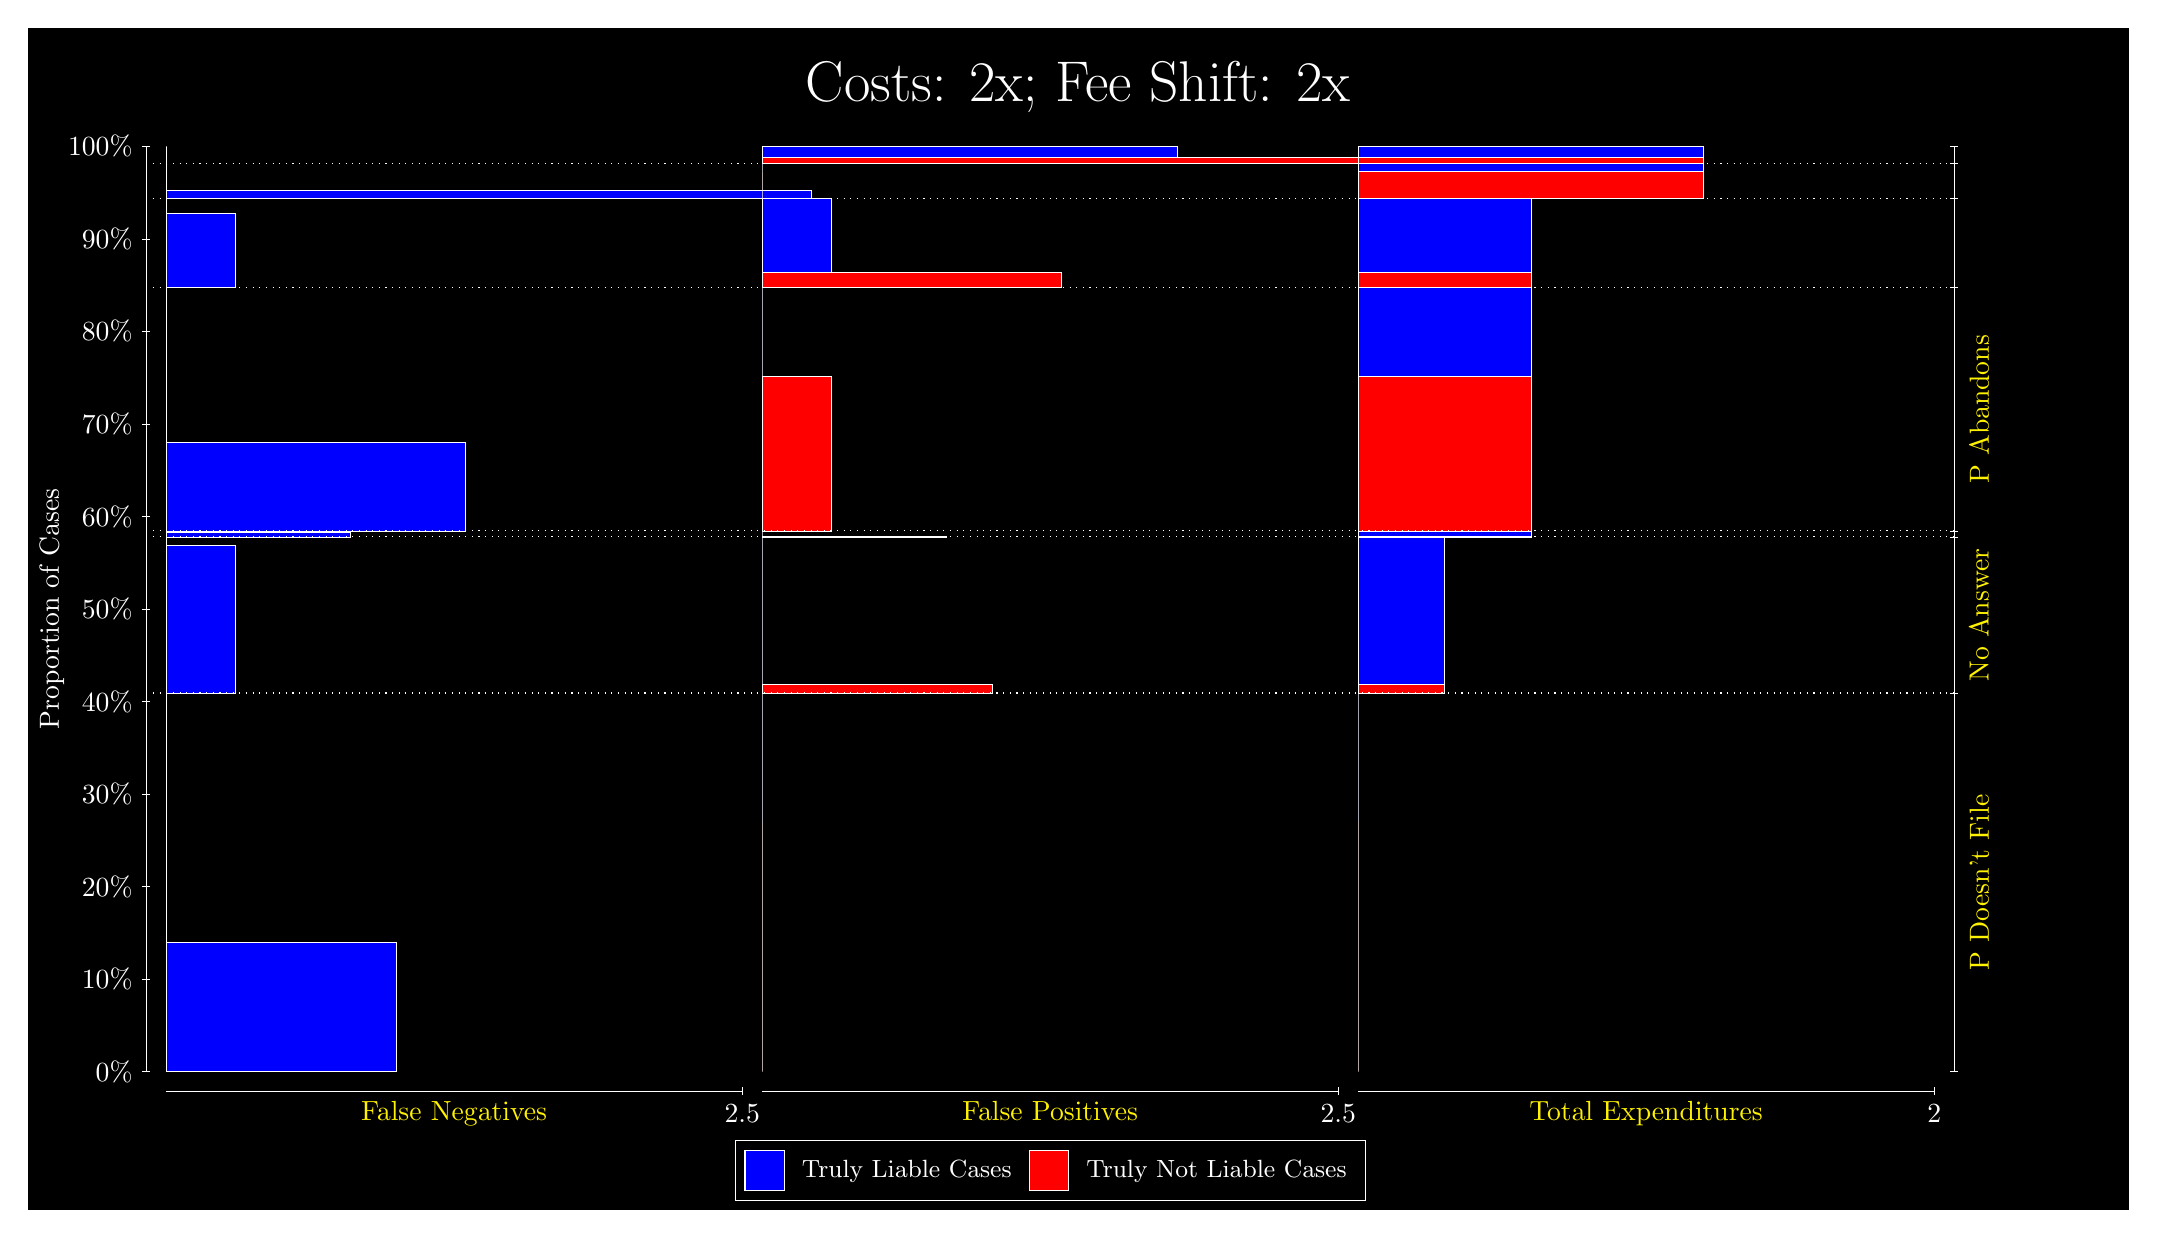
\begin{tikzpicture}
\draw[fill=black] (0,0) rectangle (26.667,15);
\draw[text=white] (0,13.5) rectangle (26.667,15) node[midway] {\huge Costs: 2x; Fee Shift: 2x};
\draw[white, very thin] (1.5,1.75) -- (1.5,13.5);
\node[rotate=90, text=white, anchor=center] at (0.3, 7.625) {Proportion of Cases};
\draw[white, very thin] (1.45,1.75) -- (1.55,1.75);
\node[text=white, anchor=east] at (1.45, 1.75) {0\%};
\draw[white, very thin] (1.45,2.925) -- (1.55,2.925);
\node[text=white, anchor=east] at (1.45, 2.925) {10\%};
\draw[white, very thin] (1.45,4.1) -- (1.55,4.1);
\node[text=white, anchor=east] at (1.45, 4.1) {20\%};
\draw[white, very thin] (1.45,5.275) -- (1.55,5.275);
\node[text=white, anchor=east] at (1.45, 5.275) {30\%};
\draw[white, very thin] (1.45,6.45) -- (1.55,6.45);
\node[text=white, anchor=east] at (1.45, 6.45) {40\%};
\draw[white, very thin] (1.45,7.625) -- (1.55,7.625);
\node[text=white, anchor=east] at (1.45, 7.625) {50\%};
\draw[white, very thin] (1.45,8.8) -- (1.55,8.8);
\node[text=white, anchor=east] at (1.45, 8.8) {60\%};
\draw[white, very thin] (1.45,9.975) -- (1.55,9.975);
\node[text=white, anchor=east] at (1.45, 9.975) {70\%};
\draw[white, very thin] (1.45,11.15) -- (1.55,11.15);
\node[text=white, anchor=east] at (1.45, 11.15) {80\%};
\draw[white, very thin] (1.45,12.325) -- (1.55,12.325);
\node[text=white, anchor=east] at (1.45, 12.325) {90\%};
\draw[white, very thin] (1.45,13.5) -- (1.55,13.5);
\node[text=white, anchor=east] at (1.45, 13.5) {100\%};

\draw[white, very thin] (24.457,1.75) -- (24.457,13.5);
\draw[white, very thin] (24.407,1.75) -- (24.507,1.75);
\node[anchor=west] at (24.407, 1.75) {};
\draw[white, very thin] (24.407,6.5568) -- (24.507,6.5568);
\node[anchor=west] at (24.407, 6.5568) {};
\draw[white, very thin] (24.407,8.5396) -- (24.507,8.5396);
\node[anchor=west] at (24.407, 8.5396) {};
\draw[white, very thin] (24.407,8.6163) -- (24.507,8.6163);
\node[anchor=west] at (24.407, 8.6163) {};
\draw[white, very thin] (24.407,11.705) -- (24.507,11.705);
\node[anchor=west] at (24.407, 11.705) {};
\draw[white, very thin] (24.407,12.835) -- (24.507,12.835);
\node[anchor=west] at (24.407, 12.835) {};
\draw[white, very thin] (24.407,13.284) -- (24.507,13.284);
\node[anchor=west] at (24.407, 13.284) {};
\draw[white, very thin] (24.407,13.5) -- (24.507,13.5);
\node[anchor=west] at (24.407, 13.5) {};

\draw[white, very thin, fill=blue] (1.75,1.75) rectangle (4.6775,3.3858);
\draw[white, very thin, fill=red] (1.75,3.3858) rectangle (1.75,6.5568);
\draw[white, very thin, fill=blue] (1.75,6.5568) rectangle (2.6283,8.4274);
\draw[white, very thin, fill=red] (1.75,8.4274) rectangle (1.75,8.5396);
\draw[white, very thin, fill=blue] (1.75,8.5396) rectangle (4.092,8.6032);
\draw[white, very thin, fill=red] (1.75,8.6032) rectangle (1.75,8.6163);
\draw[white, very thin, fill=blue] (1.75,8.6163) rectangle (5.5558,9.744);
\draw[white, very thin, fill=red] (1.75,9.744) rectangle (1.75,11.705);
\draw[white, very thin, fill=blue] (1.75,11.705) rectangle (2.6283,12.645);
\draw[white, very thin, fill=red] (1.75,12.645) rectangle (1.75,12.835);
\draw[white, very thin, fill=blue] (1.75,12.835) rectangle (9.9471,12.938);
\draw[white, very thin, fill=red] (1.75,12.938) rectangle (1.75,13.284);
\draw[white, very thin, fill=red] (1.75,13.284) rectangle (1.75,13.366);
\draw[white, very thin, fill=blue] (1.75,13.366) rectangle (1.75,13.5);
\draw[white, very thin, fill=red] (9.3189,1.75) rectangle (9.3189,4.921);
\draw[white, very thin, fill=blue] (9.3189,4.921) rectangle (9.3189,6.5568);
\draw[white, very thin, fill=red] (9.3189,6.5568) rectangle (12.246,6.669);
\draw[white, very thin, fill=blue] (9.3189,6.669) rectangle (9.3189,8.5396);
\draw[white, very thin, fill=red] (9.3189,8.5396) rectangle (11.661,8.5527);
\draw[white, very thin, fill=blue] (9.3189,8.5527) rectangle (9.3189,8.6163);
\draw[white, very thin, fill=red] (9.3189,8.6163) rectangle (10.197,10.577);
\draw[white, very thin, fill=blue] (9.3189,10.577) rectangle (9.3189,11.705);
\draw[white, very thin, fill=red] (9.3189,11.705) rectangle (13.125,11.895);
\draw[white, very thin, fill=blue] (9.3189,11.895) rectangle (10.197,12.835);
\draw[white, very thin, fill=red] (9.3189,12.835) rectangle (9.3189,13.181);
\draw[white, very thin, fill=blue] (9.3189,13.181) rectangle (9.3189,13.284);
\draw[white, very thin, fill=red] (9.3189,13.284) rectangle (17.516,13.366);
\draw[white, very thin, fill=blue] (9.3189,13.366) rectangle (14.588,13.5);
\draw[white, very thin, fill=red] (16.888,1.75) rectangle (16.888,4.921);
\draw[white, very thin, fill=blue] (16.888,4.921) rectangle (16.888,6.5568);
\draw[white, very thin, fill=red] (16.888,6.5568) rectangle (17.986,6.669);
\draw[white, very thin, fill=blue] (16.888,6.669) rectangle (17.986,8.5396);
\draw[white, very thin, fill=red] (16.888,8.5396) rectangle (19.083,8.5527);
\draw[white, very thin, fill=blue] (16.888,8.5527) rectangle (19.083,8.6163);
\draw[white, very thin, fill=red] (16.888,8.6163) rectangle (19.083,10.577);
\draw[white, very thin, fill=blue] (16.888,10.577) rectangle (19.083,11.705);
\draw[white, very thin, fill=red] (16.888,11.705) rectangle (19.083,11.895);
\draw[white, very thin, fill=blue] (16.888,11.895) rectangle (19.083,12.835);
\draw[white, very thin, fill=red] (16.888,12.835) rectangle (21.279,13.181);
\draw[white, very thin, fill=blue] (16.888,13.181) rectangle (21.279,13.284);
\draw[white, very thin, fill=red] (16.888,13.284) rectangle (21.279,13.366);
\draw[white, very thin, fill=blue] (16.888,13.366) rectangle (21.279,13.5);
\draw[white, dotted] (1.5,6.5568) -- (24.457,6.5568);
\draw[white, dotted] (1.5,8.5396) -- (24.457,8.5396);
\draw[white, dotted] (1.5,8.6163) -- (24.457,8.6163);
\draw[white, dotted] (1.5,11.705) -- (24.457,11.705);
\draw[white, dotted] (1.5,12.835) -- (24.457,12.835);
\draw[white, dotted] (1.5,13.284) -- (24.457,13.284);
\draw[white, very thin] (1.75,1.5) -- (9.0689,1.5);
\node[text=yellow, anchor=north] at (5.4094, 1.5) {False Negatives};
\draw[white, very thin] (9.0689,1.45) -- (9.0689,1.55);
\node[text=white, anchor=north] at (9.0689, 1.45) {2.5};

\draw[white, very thin] (9.3189,1.5) -- (16.638,1.5);
\node[text=yellow, anchor=north] at (12.978, 1.5) {False Positives};
\draw[white, very thin] (16.638,1.45) -- (16.638,1.55);
\node[text=white, anchor=north] at (16.638, 1.45) {2.5};

\draw[white, very thin] (16.888,1.5) -- (24.207,1.5);
\node[text=yellow, anchor=north] at (20.547, 1.5) {Total Expenditures};
\draw[white, very thin] (24.207,1.45) -- (24.207,1.55);
\node[text=white, anchor=north] at (24.207, 1.45) {2};

\node[text=yellow, centered, rotate=90] at (24.777, 4.1534) {P Doesn't File};
\node[text=yellow, centered, rotate=90] at (24.777, 7.5482) {No Answer};

\node[text=yellow, centered, rotate=90] at (24.777, 10.16) {P Abandons};




\draw (12.978300999999998,1.5) node[draw=none] (baseCoordinate) {};
\begin{scope}[align=center]
        \matrix[scale=0.5, draw=white, below=0.5cm of baseCoordinate, nodes={draw}, column sep=0.1cm]{
            \node[rectangle, draw, minimum width=0.5cm, minimum height=0.5cm, fill=blue] {}; &
            \node[draw=none, font=\small, text=white] (B) {Truly Liable Cases}; &
            \node[rectangle, draw, minimum width=0.5cm, minimum height=0.5cm, fill=red] {}; &
            \node[draw=none, font=\small, text=white] (B) {Truly Not Liable Cases}; \\
            };
\end{scope}

\end{tikzpicture}
\end{document}